% fig_dt_fgfm_tracking.tex
% TR-44: f_gfm estimation accuracy via I2/I1 ratio method
%
% Data from Study C:
%   True f_gfm: 0.00  0.25  0.34  0.50  0.75  1.00
%   Est. f_gfm: 0.015 0.232 0.357 0.527 0.758 1.000
%   Error:      0.015 0.018 0.017 0.027 0.008 0.000

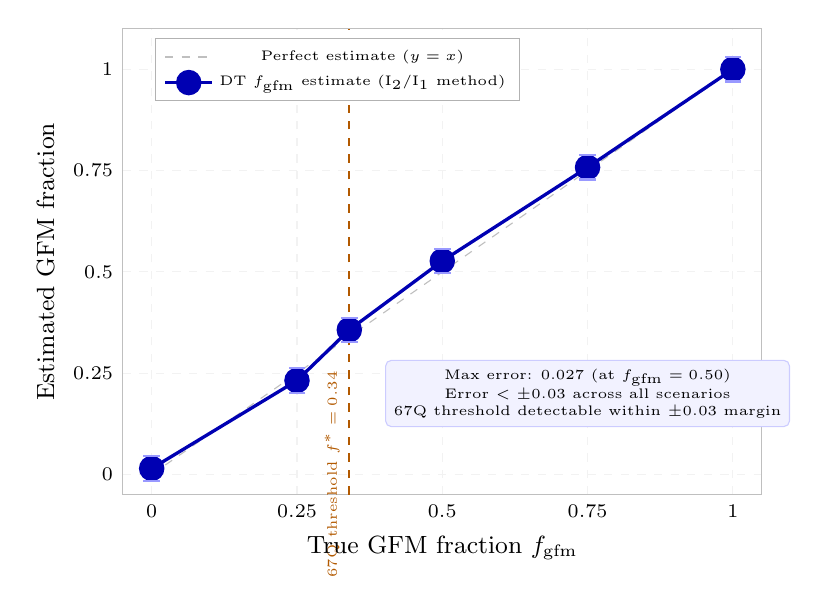
\begin{tikzpicture}
\begin{axis}[
  name         = fgfmax,
  width        = 0.80\textwidth,
  height       = 7.5cm,
  xlabel       = {True GFM fraction $f_\mathrm{gfm}$},
  ylabel       = {Estimated GFM fraction},
  xlabel style = {font=\small},
  ylabel style = {font=\small},
  xmin=-0.05, xmax=1.05,
  ymin=-0.05, ymax=1.10,
  xtick        = {0,0.25,0.50,0.75,1.00},
  ytick        = {0,0.25,0.50,0.75,1.00},
  xticklabel style={font=\scriptsize},
  yticklabel style={font=\scriptsize},
  tick style   = {draw=none},
  axis line style={gray!50},
  grid         = major,
  grid style   = {gray!10, dashed},
  legend style = {at={(0.05,0.98)}, anchor=north west, font=\tiny,
                  draw=gray!60, fill=white},
  clip=false,
]

%% Perfect reference line
\addplot[gray!50, thin, dashed]
  coordinates {(0,0) (1.0,1.0)};
\addlegendentry{Perfect estimate ($y=x$)}

%% DT estimates
\addplot[blue!70!black, very thick, mark=*, mark size=4pt]
  coordinates {
    (0.00, 0.015)
    (0.25, 0.232)
    (0.34, 0.357)
    (0.50, 0.527)
    (0.75, 0.758)
    (1.00, 1.000)
  };
\addlegendentry{DT $f_\mathrm{gfm}$ estimate (I$_2$/I$_1$ method)}

%% Error bars (±0.03 bound)
\addplot[blue!40, only marks, mark=-, mark size=3pt, thick]
  coordinates {
    (0.00, 0.015-0.03) (0.25, 0.232-0.03) (0.34, 0.357-0.03)
    (0.50, 0.527-0.03) (0.75, 0.758-0.03) (1.00, 1.000-0.03)
  };
\addplot[blue!40, only marks, mark=-, mark size=3pt, thick]
  coordinates {
    (0.00, 0.015+0.03) (0.25, 0.232+0.03) (0.34, 0.357+0.03)
    (0.50, 0.527+0.03) (0.75, 0.758+0.03) (1.00, 1.000+0.03)
  };

%% 67Q activation threshold
\draw[orange!70!black, thick, dashed]
  (axis cs:0.34, -0.05) -- (axis cs:0.34, 1.10);
\node[orange!70!black, font=\tiny, rotate=90, anchor=south]
  at (axis cs:0.34, 0.00) {67Q threshold $f^*=0.34$};

%% Annotation
\node[draw=blue!20, fill=blue!5, rounded corners=2pt,
      font=\tiny, inner sep=3pt, align=center]
  at (axis cs:0.75, 0.20)
  {Max error: 0.027 (at $f_\mathrm{gfm}=0.50$)\\
   Error $<\pm0.03$ across all scenarios\\
   67Q threshold detectable within $\pm0.03$ margin};

\end{axis}
\end{tikzpicture}
